% LaTeX Template for IT3162 Project Report, Version 1.0
% Created by: T. Jeyamugan


\documentclass[12pt, a4paper]{report}
\usepackage[pdftex]{graphicx} %for embedding images
\usepackage{url} %for proper url entries
% \usepackage[bookmarks, colorlinks=false, pdfborder={0 0 0}, pdftitle={<pdf title here>}, pdfauthor={<author's name here>}, pdfsubject={<subject here>}, pdfkeywords={<keywords here>}]{hyperref} %for creating links in the pdf version and other additional pdf attributes, no effect on the printed document

\usepackage[colorlinks]{hyperref}
\renewcommand*{\contentsname}{\hyperlink{contents}{Contents}}
\renewcommand*{\thepage}{\hyperref[contents]{\arabic{page}}}

\begin{document}
\renewcommand\bibname{References} %Renames "Bibliography" to "References" on ref page

\pagenumbering{roman} %numbering before main content starts
%Include: title, acknowledgement, dedication, tables, etc

%%%%%%%%%%%%%%%%%%%%%%%%%%%%%%%%%%%% Title page
\begin{titlepage}

\begin{center}

% Title
\Large \textbf {ElderCare Connect}\\
Progressive Web Application to Support Elderly Individuals Living Alone\\%\\[0.5in]

\vspace{1in}%


\normalsize by \\%
\vspace{1em}
\textup{\large {\bf Group 01 }\\}
 \vspace{1in}%


 \large \emph{Submitted in partial fulfilment of the requirement
for the degree of Bachelor of Science in Information Technology}
\vspace{2.5in}




\vspace{1em}
Department of Physical Science\\
Faculty of Applied Science\\
University of Vavuniya\\
% \vspace{1em}


% \vspace{.1in}
% \date{}\\


\vfill

March, 2025

\end{center}

\end{titlepage}

%%%%%%%%%%%%%%%%%%%%%%%%%%%%%%%%%%%%%%%%%%%%%%%%%%%%%%%%%%%%%%%%%%



%%%%%%%%%%%%%%%%%%%%%%%%%%%%%%%%%%%%%%      declaration
\cleardoublepage
\addcontentsline{toc}{chapter}{Declaration}
\chapter*{Declaration}
We Group 01 do hereby declare that this Project Report is original and has not been published and/or submitted for any other degree award to any other University before.


\begin{table}[!ht]
\centering
\resizebox{\textwidth}{!}{%
\begin{tabular}{|l|l|l|l|}
\hline
\textbf{\#} & \textbf{Names}  & \textbf{Registration Number} & \textbf{Signature} \\ \hline
1 & S.A.C.S. Indrejith          & 2020/ICT/65         &           \\ \hline
2 & H.D.S. Perera               & 2020/ICT/91         &          \\ \hline
3 & L.A.M. Lakmini              & 2020/ICT/44         &          \\ \hline
4 & H. Thavarajah               & 2020/ICT/120        &          \\ \hline
5 & C.G.H.P.L. Chandrasekara    & 2020/ICT/69         &          \\ \hline
6 & G. Lakashna                 & 2020/ICT/83         &          \\ \hline
7 & B.M. Imran                  & 2020/ICT/02         &          \\ \hline

\end{tabular}%
}
\end{table}
\vspace{0.5in}
\noindent
Date: ---------------\\



\newpage
%%%%%%%%%%%%%%%%%%%%%%%%%%%%%%%%%%%%%%%%%%%%%%%%%%%%%%%%%%%%%%%%%%%%%%%

%%%%%%%%%%%%%%%%%%%%%%%%%%%%%%%%%%%%%%%%%%%%%%%%%%%  Supervisor's   Approval
\cleardoublepage
\addcontentsline{toc}{chapter}{Approval}
\chapter*{Approval}
This Project Report has been submitted for examination with the approval of the supervisor/ following supervisors.

\vspace{1.0em}
\noindent
Signature:          \hspace{4in} Date: \\

\vspace{2.0em}

\noindent
Mr. K. Mathanaharan \\

\vspace{2.0em}
\noindent

\newpage
%%%%%%%%%%%%%%%%%%%%%%%%%%%%%%%%%%%%%%%%%%%%%%%%%       Abstract
\cleardoublepage
\addcontentsline{toc}{chapter}{Abstract}
\chapter*{Abstract}
ElderCare Connect is a Progressive Web Application (PWA) designed to enhance the safety, health monitoring, and social well-being of elderly individuals living alone. The elderly population faces significant challenges including medical emergencies, falls, and social isolation, which can lead to delayed treatment and deteriorating mental health. This application addresses these concerns by providing real-time health monitoring through integration with APIs like Google Fit, emergency response features with instantaneous alerts to caregivers or emergency services, and social engagement tools to combat isolation. Leveraging PWA technology, ElderCare Connect delivers native app-like experiences across multiple devices while maintaining offline functionality and requiring no app store installation.The application prioritizes user-friendly interface design with accessibility features for elderly users, robust security measures to protect sensitive health data, and scalable architecture to support growing user needs. By empowering elderly users to maintain independence while offering peace of mind to family members and caregivers, ElderCare Connect aims to improve quality of life, reduce hospitalization rates, and enhance the emotional resilience of elderly individuals living alone, ultimately promoting dignified and safe aging at home.




\newpage
%%%%%%%%%%%%%%%%%%%%%%%%%%%%%%%%%%%%%%%%%%%%%%%%%       acknowledgement
\cleardoublepage
\addcontentsline{toc}{chapter}{Acknowledgement}
\chapter*{Acknowledgement}
We are deeply indebted to our project supervisor Mr. K. Mathanaharan whose unlimited steadfast support and inspirations have made this project a great success. In a very special way, we thank him for every support he has rendered unto us to see that we succeed in this challenging study.

Special thanks go to our friends and families who have contained the hectic moments and stress we have been through during the course of the research project.

We thank the University of Vavuniya for giving us the grand opportunity to work as a team which has indeed promoted our team work spirit and communication skills. We also thank the individual group members for the good team spirit and solidarity.

% \newpage
% %%%%%%%%%%%%%%%%%%%%%%%%%%%%%%%%%%%%%%%%%%%%%%%%%%%%%%%%%%%%%%%%%%%%%%%%


\tableofcontents
\listoffigures
% \listoftables

\newpage
\pagenumbering{arabic} %reset numbering to normal for the main content
%%%%%%%%%%%%%%%%%%%  Intro   %%%%%%%%%%%%%%%%%%%
\chapter{Introduction}
Elderly individuals who live alone face significant health and safety challenges, including medical emergencies, falls, and feelings of isolation. Due to the lack of immediate assistance, these incidents can lead to delayed medical attention and complications. Furthermore, isolation can negatively affect their mental and emotional health. The absence of regular check-ins and health tracking increases the risk of undetected health deterioration.\\

The project aims to develop a Progressive Web Application (PWA) designed to enhance the safety, health monitoring, and social well-being of elderly individuals living alone. Through tracking real-time health (using APIs like Google Fit), the app will ensure caregivers/family members can monitor their health status from a distance.\\

The ElderCare Connect will function across multiple devices (desktops, smartphones, and tablets) with native app-like experiences, providing real-time health monitoring, emergency alerts, and social engagement features. Push notifications will ensure immediate attention during emergencies. Messaging features will help elderly connected with family, friends, and caregivers, mitigating loneliness and providing emotional support with PWA advantages. 
\section{Background}

In recent decades, smartphones have significantly changed the way we live. In terms of the health sector, elderly individuals now have greater access to health information and can enhance the convenience of managing their medical care through mobile applications. Several studies have shown the positive impact of mobile health interventions in managing lifestyle factors such as improving diet, quitting smoking, and increasing physical activity, as well as controlling chronic conditions like diabetes and hypertension. This change has also influenced the relationship between patients and their general practitioners.\\

Moreover, there has been increasing concern regarding the rising number of elderly individuals, particularly those living alone due to the population aging across the globe. This demographic group faces great challenges, including high health risks, social disconnectedness, and slow responses in case of emergencies that may endanger their lives. Considering that such a severe future scenario would likely occur much faster than a call for help or even faster than some normal medical conditions, there is a need for solutions that can protect the elderly, particularly those without nearby family members, from possible future threats.
\section{Problem Statement}
Elderly individuals who live alone often face significant challenges. In the event of an emergency, such as a fall or a sudden health complication, immediate assistance may not be available, potentially leading to severe consequences. Falls, in particular, can result in serious injuries, while unmanaged chronic conditions like diabetes require continuous monitoring to prevent critical health issues.\\

Social isolation is another major concern. Limited interaction with others can lead to feelings of loneliness and depression, which may negatively impact cognitive function and memory. As a result, some elderly individuals may neglect essential healthcare needs, such as attending medical appointments or adhering to prescribed medications.\\

While various mobile applications are available to assist older adults, they often lack comprehensive functionality. Many are designed for specific tasks, such as health monitoring, without integrating other essential features like emergency assistance or family communication. Additionally, these applications are frequently challenging to navigate, with small buttons, complex interfaces, and unclear instructions, making them less accessible for elderly users.\\

That's why we need a better app that is made just for older people who live alone. It needs to watch their health, call for help when they need it, and let them talk to family and friends.\\

ElderCare Connect will be a solution for this. It will use special sensors to watch their health and send alerts if something is wrong. It will have big, easy-to-see buttons and words. It will work even if they don't have internet all the time.\\
By making this app, we can help older people live safer, healthier, and happier lives. Their families can also feel better knowing they are okay.
\subsection{Main Objective}

Our primary objective is to develop Elder Care Connect, a specialized application designed to support independent elderly individuals. The application aims to enhance safety protocols, facilitate health monitoring, and promote social connectivity for seniors living alone.\\

The Elder Care Connect application will incorporate the following key functionalities:


\subsection{Scope of the Study}

This section delineates the parameters and limitations of the ElderCare Connect project, establishing clear boundaries for development and implementation.

\subsubsection*{Target Demographic:}
\begin{itemize}
    \item The application is designed for semi-independent elderly individuals requiring minimal assistance with safety and health monitoring.
    \item Users should possess basic technological literacy for interaction with mobile devices and tablets.
    \item The solution is not intended for individuals requiring intensive medical supervision or residing in assisted living facilities.
\end{itemize}

\subsubsection*{Application Functionality:}
\begin{itemize}
    \item Health monitoring through wearable device integration.
    \item Emergency alert system for crisis situations.
    \item Social connectivity tools to mitigate isolation.
    \item Cross-platform compatibility for mobile devices, tablets, and desktop computers.
    \item Offline functionality during connectivity interruptions.
    \item Secure health data management and storage.
\end{itemize}

\subsubsection*{Technical Implementation:}
\begin{itemize}
    \item Development utilizing current programming languages and frameworks.
    \item Integration with commercially available wearable biometric devices.
    \item Cloud-based data storage with appropriate security protocols.
    \item Compliance with relevant data protection and privacy regulations.
\end{itemize}

\subsubsection*{Geographic Implementation:}
\begin{itemize}
    \item Initial deployment in a controlled test region for validation purposes.
    \item Multilingual and multicultural adaptability for broader implementation.
\end{itemize}

\subsubsection*{Project Timeline:}
\begin{itemize}
    \item Structured development schedule with defined milestones.
    \item Focus on core functionality for initial release with planned feature expansion in subsequent iterations.
\end{itemize}

\subsubsection*{Exclusions:}
\begin{itemize}
    \item Development of proprietary medical hardware devices.
    \item Direct provision of medical services.
\end{itemize}
\section{Significance of the Study}
ElderCare Connect is important because it can make a big difference in the lives of older people, their families, and the community. It can help older people stay healthy, safe, and connected, and it can give their families peace of mind.\\

\textbf{How It Helps Older People:}
\begin{itemize}
    \item Better Life: It helps them live a better life by watching their health, getting help fast when they need it, and talking to family and friends.
    \item Less Time in the Hospital: It can keep them from having to go to the hospital by finding problems early and helping them get help fast.
    \item Happier Feelings: It helps them feel less lonely and more connected, which makes them happier.
    \item Stay Independent: It helps them stay in their own homes longer because they have the support they need to stay safe and healthy.
\end{itemize}
\textbf{How It Helps Families:}
\begin{itemize}
    \item Peace of Mind: It gives families peace of mind knowing that their loved ones are safe and healthy.
    \item Fast Help: It makes sure they get help fast if something goes wrong.
    \item Good Communication: It helps them talk to their loved ones and stay connected.
    \item Less Worry: It takes some of the worry away because they know their loved ones have the tools they need to stay safe.
\end{itemize}
\textbf{How It Helps the Community:}
\begin{itemize}
    \item Promotes Tech for Health: It shows that technology can help older people stay healthy and safe.
    \item Sets a Good Example: It sets a good example for how to make new technology for older people.
    \item Saves Money: It can save money on healthcare by keeping older people out of the hospital.
    \item Supports Staying at Home: It helps older people stay in their own homes and communities, which is good for them and for the community.
\end{itemize}
By making ElderCare Connect, we can help older people live better, safer, and happier lives. We can also give their families peace of mind and make our community a better place for older people to live.
\newpage
%%%%%%%%%%%%%%%%%%%  Literature Review   %%%%%%%%%%%%%%%%%%%
\newpage
%%%%%%%%%%%%%%%%%%%%%%%%%%%%%%%%%%%%%%%%%%%%%%%%%%%%%%%%%%%%%%%%%%%%%%

%%%%%%%%%%%%%%%%%%%                 literature
\chapter{Literature Review}

\section{Introduction}
As per the recent litearture, aging is a universal phenomenon expected to continue 
existing for the time being. By 2013, approximately 
841 million individuals (11.7\%) had passed the age of 
60 \cite{MH17464}. Although aging cannot be prevented, better understanding by local residents can 
help them feel healthy despite functional deterioration 
and some diseases \cite{eldersHealthFactors}. As individuals age, their intrinsic capacities decline, and the risk of multi-morbidity increases, resulting in the need for ongoing monitoring or treatment \cite{xue2021intrinsic}. \\

An early study shows the factors affecting fall accidents in elderly people who live alone. According to that,\\ 
\begin{itemize}
    \item Main behavioral factors include taking medicine to treat chronic diseases, using alcoholic beverages, not exercising, wearing comfortable shoes, Inappropriate clothing. 
    \item Main environmental regularly using stairs two-story house, split-level house, light switch not nearby, mattress. 
    \item Main economic and social factors, frequently attending social events, missing home visits from the health service unit. 
    \item The main factor was caregiver. The sub-factor is living with offspring and having to live alone.
\end{itemize}
It was found that above factors are affecting the incidence of falls in elderly people who live alone
 \cite{Srenual_Kanokthet_2024}.

Moreover research articles highlight that for many countries, the emergence of an ageing population is fast becoming an increasing public health concern. Healthcare costs are continuously rising and the quality of services does not meet the needs of modern society. Remote real-time health monitoring provides one possible solution to overcoming these challenges. Constantly monitoring the
 health of elderly people via wearable devices and fitness trackers proved different avenues in facilitating Early Intervention Practices EIP and reducing release rates \cite{RemoteHealth}.\\
 
According to the recent studies,  Generally, innovative information and communication technology can play a significant role in caring for elderly patients, at their own homes or at other healthcare environments\cite{MH17464}. Over the past few decades, smartphones have fundamentally changed our daily lives. In terms of health, older adults now have more opportunities to obtain health knowledge and improve the convenience of their medical treatment using apps. Several studies have demonstrated the effectiveness of mobile health interventions in the management of lifestyle factors (eg, improving dietary habits, quitting smoking, and increasing physical activity) and chronic diseases (eg, diabetes, Parkinson disease, high blood pressure) \cite{chinese_survey}.  In 2019, the adoption rate of smartphones by older adults aged 55–91 years was 40–68 \% text, mHealth is a promising tool for promoting healthy aging through evidence-based self-management interventions that help older adults maintain functional ability and independence \cite{Liaw-2019}. The effectiveness of mHealth in promoting healthy behavior and managing chronic diseases has been proven. Usability is considered a vital factor influencing the adoption of mHealth by the elderly which is defined as “the extent to which a system can be used by specified users to achieve specified goals with effectiveness, efficiency and satisfaction in a specified context of use” \cite{eldersHealthFactors}. As mHealth technologies grow, emerging applications of the technologies will enable life-changing uses for the elderly population. The application of mHealth has the potential to improve outcomes and change the course of health care as it is provided today \cite{mHealthforAgingPopulation}.\\

 The growing elderly population, accompanied by the increasing prevalence of chronic diseases associated with aging, will have profound implications for the health care system for decades to come. Therefore, it is becoming essential to engage technologies such as healthcare sensors and wearable with our healthcare systems, in order to have a safer and convenient environment for everyone to live in \cite{RemoteHealth}.
\\

Furthermore there are more projects which has done regarding this title under several categories. Recent researches identifies them as, The project Aware Home uses a wide variety of sensors, covering from specifically designed smart floors to more typical video and ultrasonic  sensors, together with social robots to monitor and help older adults. The Ubiquitous  HomeProject is also centred in residents monitoring through a robot, which includes a dialogue based interface and operates as an intermediate platform between the smart home and the end users. In addition, some projects have focused on the monitoring patients
suffering from a chronic disease, such as CASAS project, which use the smart-homes environment to monitor patients suffering from dementia, which is similar to ENABLE
project with the goal of giving them more autonomy in their lives. While, DOMUS and IMMED projects focus on behaviour recognition for patients suffering from Alzheimer disease. Grenoble Health Smart Home proposed a set of tools to measure patients activity in hospitals via several indicators of their activities in daily living, mobility, and repartition of stays and displacements. In the Gloucester Smart House project, a telehealth system was designed, based on lifestyle monitoring, with the pretension of continuously gathering information about the patients activity during daily routines \cite{RemoteHealth}. \\

In addition to that past literature has identified that Wearable sensors and health-monitoring devices, including heart rate sensors, pulse  sensors, oxygen sensors, and blood pressure sensors, play a crucial role in remote health monitoring systems, whether in open or closed environments, for observing patients. These sensors detect any abnormalities in the patient’s behavior, prompting immediate action from caregivers or doctors, enabling them to take necessary measures promptly to address the situation. In addition to these wearable sensors, vision-based sensors are also employed to monitor the health conditions of patients. For instance, a camera mounted near the patient’s vicinity keeps track of the patient’s movement. If the system detects any abnormal movement by the patient, it promptly triggers an alarm to notify the caretaker. By combining wearable and vision-based sensors, healthcare providers can comprehensively monitor and respond to the well-being of patients in real-time \cite{ASurvey}.\\

Throughout the past literature, a common problem found while researching was the lack of feature rich applications available in Sri Lanka. Though there are applications available with appealing features 
they are mainly available in the other countries. Therefore the aim of this project is to provide an application that both the family and elderly person can interact with enabling elder care.


\newpage
\newpage
%%%%%%%%%%%%%%%%%%%  methodology   %%%%%%%%%%%%%%%%%%%

%%%%%%%%%%%%%%%%%%%%%%%%%%%%%%%%%%%%%%%%%%%%%%%%%%%%%%%%%%%%%%%%%%

\newpage
\chapter{Methodology}


\section{Introduction}
ElderCare Connect is a Progressive Web App (PWA) designed to improve the safety, health monitoring, and social engagement of elderly individuals living alone. The app enables real-time health tracking, emergency alerts, and fosters social connections to combat loneliness among the elderly. With features like integration with Google Fit, emergency call APIs, and push notifications, the app aims to offer a comprehensive solution for elderly care.  
The app is available across multiple devices (smartphones, tablets, and desktops) without requiring installation, ensuring accessibility for elderly users who may have limited technical knowledge. Through this project, we aim to create a solution that enhances the well-being of elderly people, provides peace of mind to their families, and ensures prompt emergency response when necessary\cite{eldercare_solutions}.

\section{Importance of Implementation}
The implementation phase is the most critical in turning the conceptual design of ElderCare Connect into a fully functioning app. It is at this stage where the app's core features are developed, tested, and optimized for real-world use. Effective implementation ensures that the app is functional, secure, and scalable, fulfilling its purpose of supporting elderly individuals.  
This phase involves integrating various technologies and services, such as health tracking with wearable devices, push notifications for emergencies, and secure authentication with JWT. It also includes rigorous system testing to detect and fix any issues before deployment. The implementation of these features directly impacts user experience, reliability, and the app's ability to meet its intended goals\cite{pwa_development}.

\section{Implementation Methodology}

The development of ElderCare Connect followed an Agile methodology, which allowed for iterative development and continuous feedback from stakeholders\cite{agile_manifesto}. The project was broken down into smaller, manageable tasks that were completed in sprints, ensuring that each feature was developed, tested, and integrated step by step\cite{scrum_guide}. This approach allowed the team to make improvements based on real-time feedback and user testing.

\begin{itemize}
    \item \textbf{Sprint 1:} Requirements gathering and setup of the development environment.
    \item \textbf{Sprint 2:} Frontend development (UI/UX design, layout creation using Next.js and Tailwind CSS)\cite{nextjs_docs}.
    \item \textbf{Sprint 3:} Backend development (API setup with Node.js and Express, Firebase integration for real-time notifications)\cite{nextjs_docs}.
    \item \textbf{Sprint 4:} Integration of real-time health monitoring (Google Fit)\cite{google_fit}.
    \item \textbf{Sprint 5:} Security implementation (JWT authentication, SSL encryption)\cite{jwt_handbook}.
    \item \textbf{Sprint 6:} Testing, deployment, and final refinements based on user feedback\cite{firebase_docs}.
\end{itemize}

\section{Implementation Environment}

The implementation environment for ElderCare Connect consists of various tools and technologies that support both frontend and backend development.

\subsection*{Frontend:}
\begin{itemize}
    \item \textbf{Next.js:} Chosen for its ability to build server-side rendered React applications, making the app more SEO-friendly and performant\cite{nextjs_docs}.
    \item \textbf{Tailwind CSS:} A utility-first CSS framework that enabled rapid design implementation\cite{tailwind_docs}.
\end{itemize}

\subsection*{Backend:}
\begin{itemize}
    \item \textbf{Node.js:} The backend is built with Node.js due to its non-blocking, event-driven architecture, making it ideal for real-time data handling\cite{nodejs_docs}.
    \item \textbf{Express.js:} A web application framework for Node.js, used to handle routing and middleware for API requests\cite{express_docs}.
    \item \textbf{MongoDB/Firebase:} MongoDB is used for storing user data and health records, while Firebase handles real-time notifications and authentication\cite{mongodb_docs}.
\end{itemize}

\subsection*{Other Tools:}
\begin{itemize}
    \item \textbf{Git:} Version control system for team collaboration\cite{git_docs}.
    \item \textbf{Postman:} Used for API testing during development\cite{postman_docs}.
    \item \textbf{Firebase Cloud Messaging (FCM):} For sending push notifications, emergency alerts, and real-time medication reminders\cite{firebase_fcm}.
    \item \textbf{Jest:} A testing framework used to ensure that the backend APIs function as expected\cite{jest_docs}.
\end{itemize}

\section{Tools Used}

\subsection*{Frontend:}
\begin{itemize}
    \item \textbf{Next.js:} Framework for building React-based web applications.
    \item \textbf{Tailwind CSS:} Used for creating responsive and modern designs.
    \item \textbf{Figma:} Design tool for UI/UX wireframing and prototyping.
\end{itemize}

\subsection*{Backend:}
\begin{itemize}
    \item \textbf{Node.js:} JavaScript runtime for the server-side environment.
    \item \textbf{Express.js:} Web framework for building APIs.
    \item \textbf{MongoDB/Firebase:} Database management (MongoDB for storing data, Firebase for real-time notifications and authentication).
    \item \textbf{JWT:} JSON Web Token used for secure authentication.
\end{itemize}

\subsection*{Testing:}
\begin{itemize}
    \item \textbf{Jest:} For unit and integration testing.
    \item \textbf{Postman:} For testing the backend API endpoints.
\end{itemize}

\subsection*{Version Control:}
\begin{itemize}
    \item \textbf{Git:} Used for source code management and version control, with GitHub for collaboration.
\end{itemize}

\section{\System Testing}

System testing was carried out to ensure that the ElderCare Connect app functions as expected under various conditions. The testing process included:

\begin{itemize}
    \item \textbf{Unit Testing:} Testing individual components like the login system, emergency alerts, and API endpoints using Jest\cite{jest_docs}.
    \item \textbf{Integration Testing:} Ensuring that components such as the frontend, backend, and Firebase service work seamlessly together\cite{firebase_testing}.
    \item \textbf{User Acceptance Testing (UAT):} Involving actual users to test the app’s usability and gather feedback on its features and design\cite{uat_testing}.
    \item \textbf{Performance Testing:} Checking the app's ability to handle real-time notifications and large datasets without delays\cite{performance_testing}.
    \item \textbf{Security Testing:} Ensuring that data, especially health-related data, is securely transmitted using SSL encryption, and verifying the robustness of JWT-based authentication\cite{security_testing}\cite{jwt_security}.
\end{itemize}

\section{Technical Stack}

\begin{itemize}
    \item \textbf{Frontend:} Next.js, Tailwind CSS
    \item \textbf{Backend:} Node.js, Express.js
    \item \textbf{Database:} MongoDB, Firebase
    \item \textbf{Real-Time Services:} Firebase Cloud Messaging (FCM), WebSockets
    \item \textbf{Authentication:} JWT (JSON Web Token)
    \item \textbf{Security:} SSL encryption
    \item \textbf{Testing Tools:} Jest, Postman
    \item \textbf{Version Control:} Git, GitHub
    \item \textbf{Deployment:} Firebase Hosting
\end{itemize}

\section{Gantt Chart}

\begin{figure}[htbp]
  \centering
  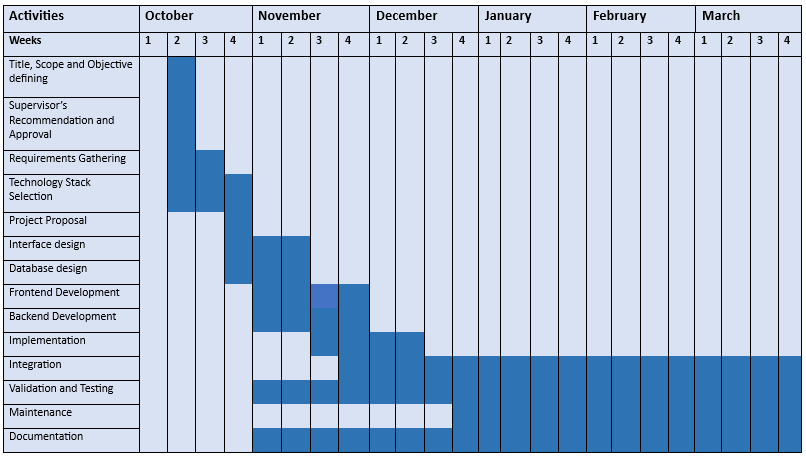
\includegraphics[width=6.4in]{ganttchart.PNG}
  \caption{Timeline}
  \label{fig:ganttchart}
\end{figure}



 



\newpage
%%%%%%%%%%%%%%%%%%%  analysis and design %%%%%%%%%%%%%%%%%%%

\chapter{System Study, Analysis and Design}

\section{Overview of the System}
The ElderCare Connect is a Progressive Web Application (PWA) designed to enhance the quality of life, safety, and well-being of elderly individuals living alone. The system leverages modern web technologies to create a responsive, accessible platform that functions across multiple devices while maintaining an app-like experience.
The system interconnects three key user groups:

    \begin{enumerate}
        \item Elderly users who are the primary beneficiaries
        \item Family members who monitor and support their elderly relatives
        \item Caregivers who provide professional assistance
    \end{enumerate}
The application integrates real-time health monitoring through google fit API, emergency response mechanisms, and social engagement features, all designed with elderly-friendly interfaces and robust security measures

\section{System Architecture}
\subsection{High-Level Architecture}
ElderCareConnect employs a multi-tier architecture consisting of:
    \begin{enumerate}
        \item \textbf{Presentation Layer:} Implemented using Next.js with Tailwind CSS for responsive and accessible user interfaces optimized for elderly users
        \item \textbf{Application Layer:} Built on Node.js and Express.js for processing business logic and handling requests
        \item \textbf{Data Layer:} Utilizing MongoDB for data persistence and Firebase for real-time features
        \item \textbf{Integration Layer:} APIs connecting to Google Fit, and emergency services
        \item \textbf{Security Layer:} JWT authentication, SSL encryption, and role-based access control
    \end{enumerate}
    % \begin{itemize}
    %         \item \textbf{Frontend: } Next.js with Tailwind CSS
    %         \item \textbf{Backend: } Node.js and Express.js
    %         \item \textbf{Database: } MongoDB
    %         \item \textbf{Real-time Services: } Firebase
    %         \item \textbf{Authentication: } JWT (JSON Web Tokens)
    % \end{itemize}

\subsection{Component Architecture}
The system is divided into five major components, each handling specific functionalities:
        \begin{enumerate}
            \item User Management Component
                \begin{itemize}
                    \item User registration and authentication
                    \item Profile management
                    \item Role-based access control (elderly users, family members, caregivers) 
                    \item User preferences and settings
                \end{itemize}
            \item Health Monitoring Component
                \begin{itemize}
                    \item Google Fit API integration
                    \item Vital signs monitoring (heart rate, blood pressure, activity levels)
                    \item Sleep pattern tracking
                \end{itemize}
            \item Emergency Response Component
                \begin{itemize}
                    \item SOS button functionality
                    \item Automated emergency alerts
                    \item GPS location tracking
                    \item Emergency contact notification system
                \end{itemize}
            \item Social Engagement Component
                \begin{itemize}
                    \item Instant messaging system
                    \item Location Sharing
                    \item Remiders Sharing
                \end{itemize}
            \item Notification and Alert System
                \begin{itemize}
                    \item Push notifications for emergencies
                    \item Medication reminders
                    \item Health check-ins
                    \item Appointment reminders
                    \item Hydration alerts
                \end{itemize}
        \end{enumerate}
\section{System Requirements}
\subsection{Functional Requirements}
\textbf{Health Monitoring} \\[0.25cm]
 The app will be able to synchronize and connect with wearable devices as well as health monitoring platform, Google Fit (Android) which are designed to monitor the heart rate of users, their activity, etc. sleep patterns, their activity levels etc. This data shall be monitored over the internet and in case of any abnormalities, such as a distinct drop in heart rate or a fainting episode, alerts will go off \cite{jmirSmartphoneHealth}. 
 \\[0.25 cm]
\textbf{Emergency Response} \\[0.25cm]
In the event of a medical emergency or situation where a patient falls, the app shall send push notifications to the emergency contacts or the caregivers who are predesignated. It is also possible for the users to use the emergency call function (with the help of a REST API) in case they feel the need for help or are unwell. \\
\\[0.25 cm]
\textbf{Social Engagement} \\[0.25cm]
Recognizing the significance of social engagement, which is crucial in enhancing the well-being of the elderly, the only such application will integrate a number of features such as instant messaging where old or elderly users can meet family members, caregivers, which will help in alleviating loneliness and associated feelings. If the elderly member is in danger this features a location sharing technique to send their location to their cared ones. This also allows the family members and caregivers to remind their lovely one’s medications hydrations and medical consultations simply contact with them. \\
\subsection{Non-functional Requirements}
\textbf{Performance:}
    \begin{itemize}
            \item The app should provide real-time monitoring and instant emergency alerts within 2 seconds of a triggering event 95\% of the time, especially during critical moments such as falls or health issues.
            \item It should handle multiple users and the input of real-time data from Google Fit Application maintaining a response time of under 1 second per device.
    \end{itemize}
\textbf{Usability:}
    \begin{itemize}
        \item The user interface should be simple and intuitive, designed with large fonts (minimum size 18pt) and easy navigation, particularly catering to elderly users with minimal technical experience (new users will be able to locate easily the primary functions such as emergency alerts, health stats, and alerts within 2 seconds).
        \item The app must be highly reliable to ensure constant monitoring and timely emergency alerts, with at least 99.9\% uptime.
        \item Emergency alert mechanisms should function with at least 98\% accuracy, even in low connectivity scenarios (1 Mbps). 
    \end{itemize}
\textbf{Security}
    \begin{itemize}
        \item Data privacy and security are critical, especially since the app deals with sensitive health information. The app must comply with healthcare privacy regulations such as HIPAA (or regional equivalents) to protect user data, as well as the Personal Data Protection Act (PDPA).
        \item Secure login and role-based access for family members and caregivers to ensure that only authorized individuals can view the health data of the elderly user.
    \end{itemize}
\textbf{Scalability}
    \begin{itemize}
        \item  The back-end should support future scalability as 100\% increase in users and data volume within one year without affecting performance metrics, handle up to 5 million records allowing additional data points (such as vital signs) as needed.
    \end{itemize}
\textbf{Maintainability}
    \begin{itemize}
        \item The system should be easy to update with new features or improvements, such as new integrations with different wearable devices or additional health monitoring features with a maximum downtime of 5 minutes per update.
    \end{itemize}
\textbf{Availability}
    \begin{itemize}
        \item  The system must ensure high availability, especially during emergencies, and maintain up-time for 24/7 real-time monitoring.
        \item  Regular maintenance or updates should not interfere with the core emergency functionality.
    \end{itemize}
\textbf{ Privacy and Security}
    \begin{itemize}
        \item As the application deals with sensitive personal health information, the app will definitely put in place stringent measures such as the use of JWT (JSON Web Tokens) for user validation and SSL which encrypts data during transfer. Such measures go a long way in securing personal health information.
    \end{itemize}
\subsection{User Requirements}
\begin{minipage}{\textwidth}
        \centering
        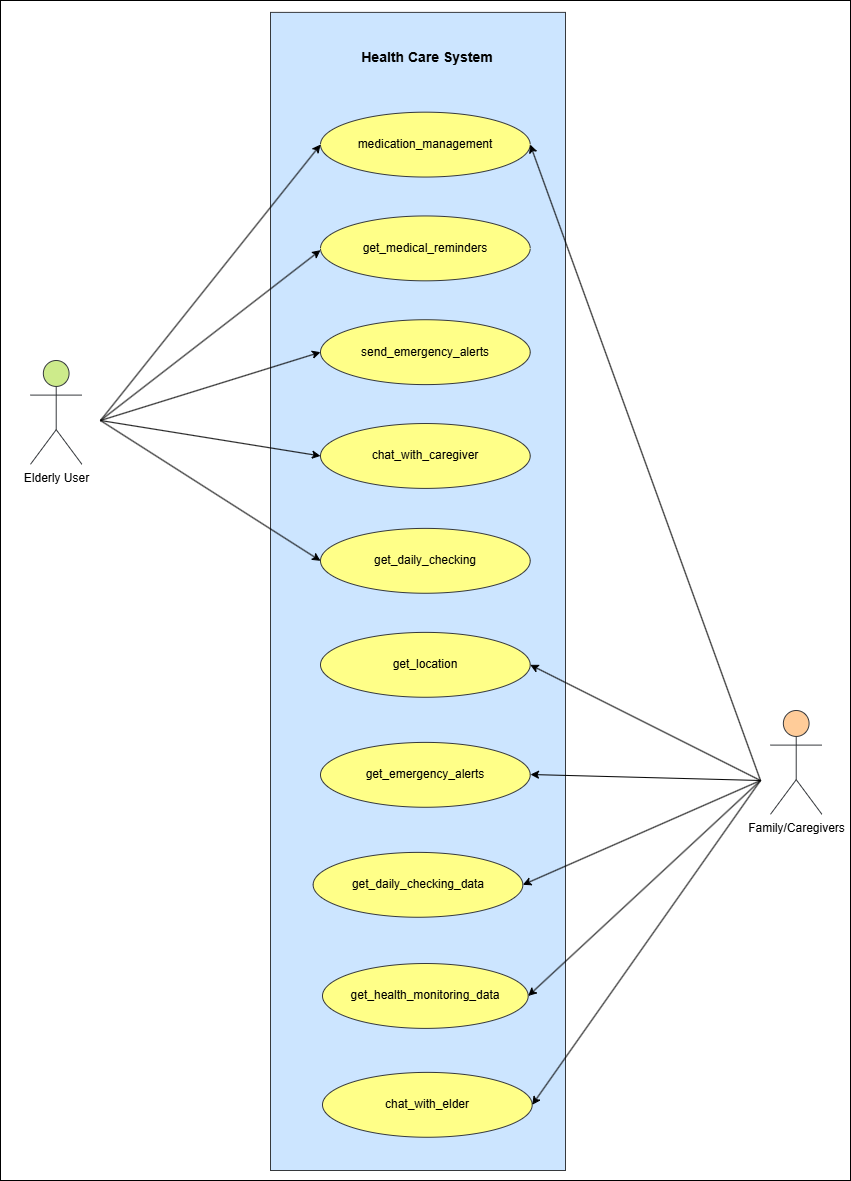
\includegraphics[width=0.9\textwidth]{usecase.drawio.png}
        \caption{Usecase}
        \label{fig:usecase}
    \end{minipage}\\
    
\textbf{\large Elderly Users} 
\begin{itemize}
    \item \textbf{Health Monitoring:} Integration with wearable devices to track vital signs like heart rate, blood pressure, and physical activity. 
    \item \textbf{Emergency Alerts:} Automatic fall detection and an SOS button for emergencies, sending alerts to family, caregivers, or emergency services.
    \item \textbf{Medication Reminders:} Notifications to take prescribed medications, reducing the risk of missed doses. 
    \item \textbf{Daily Check-ins:} Gentle reminders for users to confirm their well-being or complete a wellness survey.
    \item \textbf{Social Engagement:} Messaging, and virtual communities to reduce isolation and encourage interaction.
\end{itemize}
\textbf{\large Caregivers/family} 
\begin{itemize}
    \item \textbf{Real-time Alerts:} Immediate notifications for falls, emergencies, or missed check-ins.
    \item \textbf{Health Reports:} Weekly or monthly health reports with trends in the user's vital stats, activity levels, and overall well-being.
    \item \textbf{Location Tracking:} Real-time GPS tracking during emergencies or to ensure the user's safety.
    \item \textbf{Communication Tools:} Instant messaging to check on the elderly user.
\end{itemize}
\section{System Design Considerations} 
\begin{itemize}
    \item Front-end: Next.js with Tailwind CSS
    \item Backend: Node.js, Express.js
    \item Database: MongoDB
    \item Real-time Services: Firebase
    \item Communication: Twilio API
\end{itemize}
\section{Technology Stack}
\begin{itemize}
    \item Programming Languages: JavaScript/TypeScript
    \item Front-end Framework: Next.js
    \item Styling: Tailwind CSS
    \item Backend: Node.js, Express.js
    \item Database: MongoDB
    \item Real-time Database: Firebase
    \item Authentication: JWT
    \item APIs: Google Fit, Twilio
\end{itemize}



\newpage
%%%%%%%%%%%%%%%%%%%    presentation   %%%%%%%%%%%%%%%%%%%
\chapter{Presentation of results}
\section{Introduction}
This chapter presents a comprehensive overview of the system's results, including the user interface design, system functionalities, and the development environment used to build Elder Care Connect. The chapter is structured to provide a clear understanding of how the system operates through relevant screenshots, descriptions of core features, and an analysis of system performance. Additionally, this section discusses the tools, frameworks, and programming environments that were utilized during development, highlighting the technical aspects that contribute to the system’s efficiency and reliability.
\section{System Interfaces and User Experience}
The Elder Care Connect system has been designed with a user-centric approach, ensuring accessibility and ease of use for both elderly users and caregivers. The following subsections provide a detailed presentation of the user interfaces, highlighting key features with accompanying screenshots.
\begin{enumerate}
    \item \textbf{Login and Authentication System}
    \begin{itemize}
        \item A secure login system using google authentication and also email and password authentication with role-based access control (caregivers and elderly users).
    \end{itemize}
    \item \textbf{Dashboard Overview}
        \begin{itemize}
            \item The dashboard serves as the central hub, providing quick access to key functionalities.
            \item Features include an overview of medication schedules, chat notifications, and location tracking.
            \end{itemize}
    \item \textbf{Medication Reminder Management}
            \begin{itemize}
                \item A user-friendly interface allowing caregivers to set up medication schedules with time-based alerts.
                \item Elderly users receive visual reminders for medication intake.
            \end{itemize}
    \item \textbf{Real-Time Chat and Communication}
            \begin{itemize}
                \item Secure WebSocket-based real-time chat for seamless communication between caregivers and elderly users.
                \item Supports text, share reminders and location for enhanced interaction.
            \end{itemize}
    \item \textbf{Emergency Alerts}
                \begin{itemize}
                    \item Integrated emergency alert notifications.
                \end{itemize}             
\end{enumerate}
\section{Programming Environment and Technologies Used}
To develop the Elder Care Connect system, a modern technology stack was employed to ensure high performance, scalability, and security. The following tools and frameworks were integral to the development process:
\begin{enumerate}
    \item \textbf{Frontend Development}
        \begin{itemize}
            \item \textbf{Node.js:} Used for building a dynamic and responsive user interface with reusable components.
            \item \textbf{Tailwind CSS:} Applied for designing a visually appealing and accessible UI.
        \end{itemize}
    \item \textbf{Backend Development}
        \begin{itemize}
            \item \textbf{Node.js and Express.js:} Powering the backend API with RESTful services for seamless communication between the frontend and database.
            \item \textbf{WebSocket.io:} Used for real-time chat and live updates.
            \item \textbf{JWT (JSON Web Tokens):} Implemented for secure user authentication and authorization.
        \end{itemize}
    \item \textbf{Database Management}
    \begin{itemize}
        \item \textbf{MongoDB:} A NoSQL database used for storing user information, medication schedules, and chat history.
        \item \textbf{Firebase:} Utilized for real-time data synchronization, authentication, and cloud storage, ensuring seamless data access and backup \cite{firebase_docs}.
    \end{itemize}
    \item \textbf{Security and Data Protection}
        \begin{itemize}
            \item \textbf{Bcrypt.js:} Used for hashing user passwords to enhance security.
            \item \textbf {SSL Encryption:} Ensures secure data transmission over the network.
        \end{itemize}
\end{enumerate}
\section{Summary}
This chapter provided an in-depth overview of the Elder Care Connect system’s interfaces, functionalities, and technical implementation. Through the presentation of screenshots and descriptions, we demonstrated how the system facilitates seamless communication and care management for elderly individuals and caregivers. Furthermore, the programming environment and technology stack were detailed to highlight the system’s robust architecture and security measures. The performance evaluation results confirm the system’s reliability, scalability, and efficiency in real-world applications. These findings serve as a testament to the project’s success in addressing key challenges in elderly care and provide a foundation for future enhancements.
\newpage
%%%%%%% screenshots %%%%%%%%
\begin{figure}
    \centering
    \begin{minipage}{\textwidth}
        \centering
        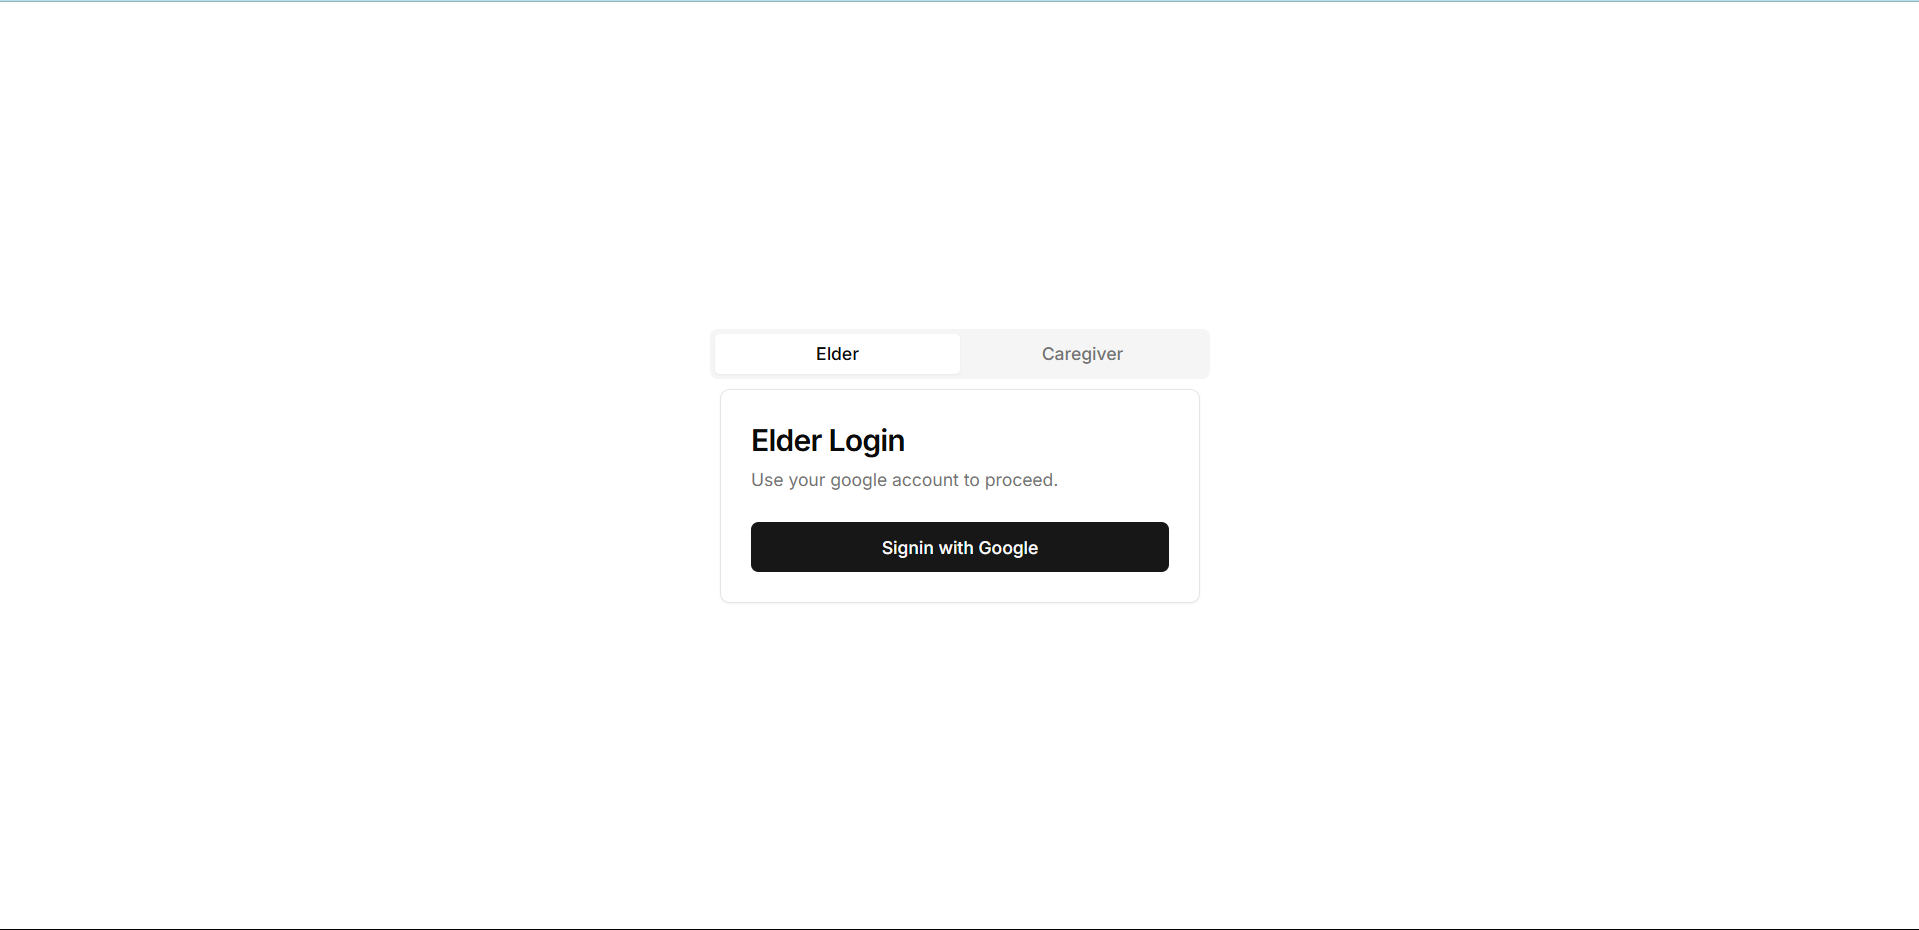
\includegraphics[width=0.9\textwidth]{login.png}
        \caption{Login Page}
        \label{fig:login}
    \end{minipage}
    \vspace{5pt}
    \begin{minipage}{\textwidth}
        \centering
        \includegraphics[width=0.9\textwidth]{dashboard.png}
        \caption{Elderly User Dashboard}
        \label{fig:elderly_dashboard}
    \end{minipage}
    \vspace{5pt}
    \begin{minipage}{\textwidth}
        \centering
       \includegraphics[width=0.9\textwidth]{dashboard.png}
        \caption{Caregiver Dashboard}
        \label{fig:caregiver_dashboard}
    \end{minipage}
    \vspace{5pt}
\end{figure}

\begin{figure}
    \centering
    \begin{minipage}{\textwidth}
        \centering
        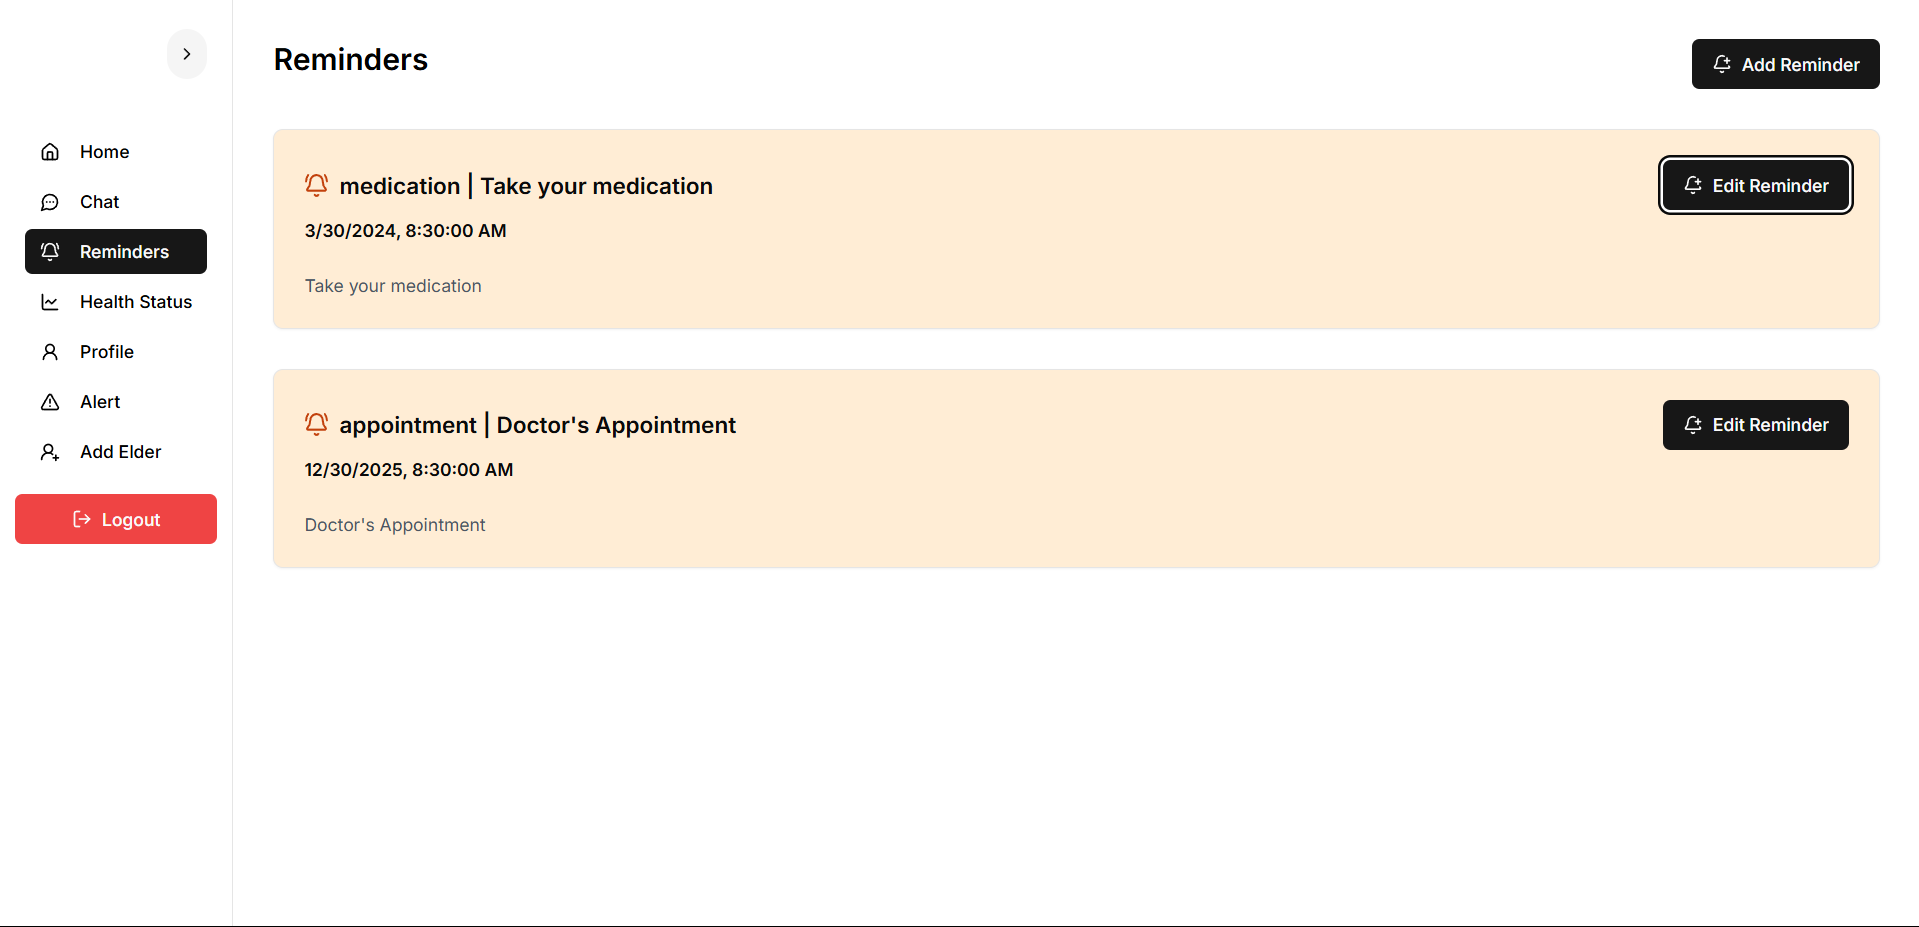
\includegraphics[width=0.9\textwidth]{reminders.png}
        \caption{Reminders\\}
        \label{fig:reminders}
    \end{minipage}
    \vspace{5pt}
    \begin{minipage}{\textwidth}
        \centering
        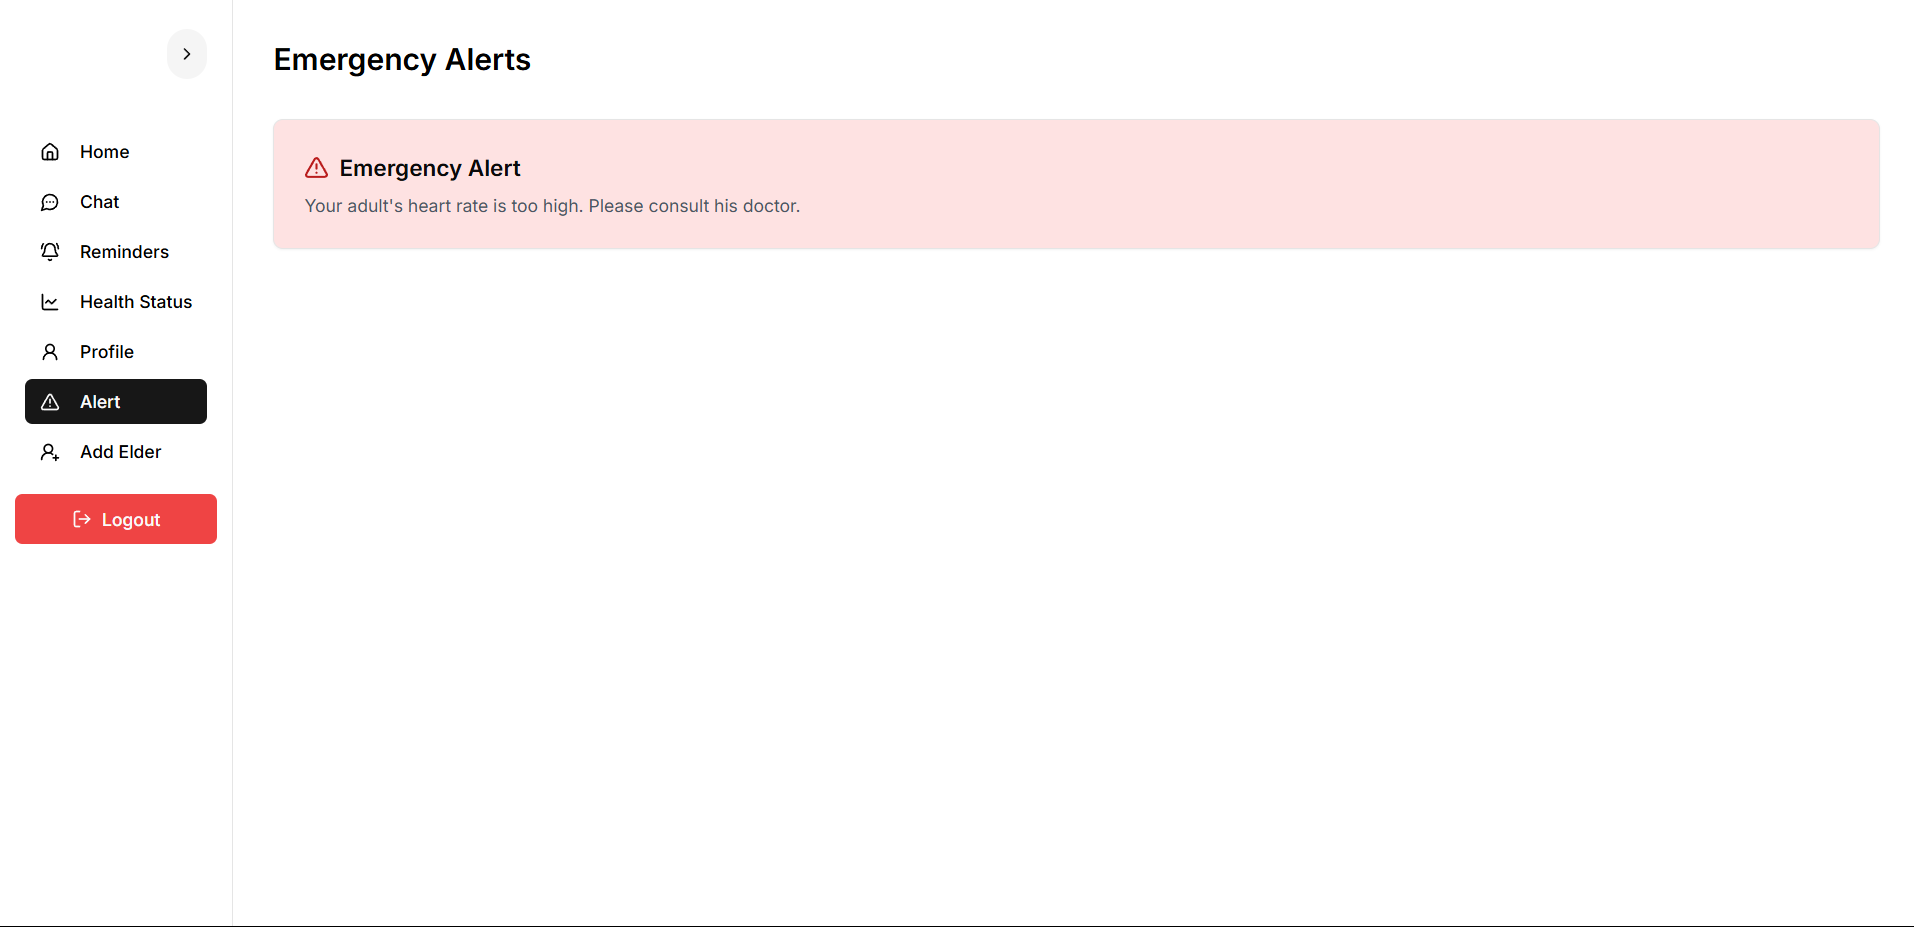
\includegraphics[width=0.9\textwidth]{alert.png}
        \caption{Alerts}
        \label{fig:alerts}
    \end{minipage}
    \vspace{5pt}
    \begin{minipage}{\textwidth}
        \centering
        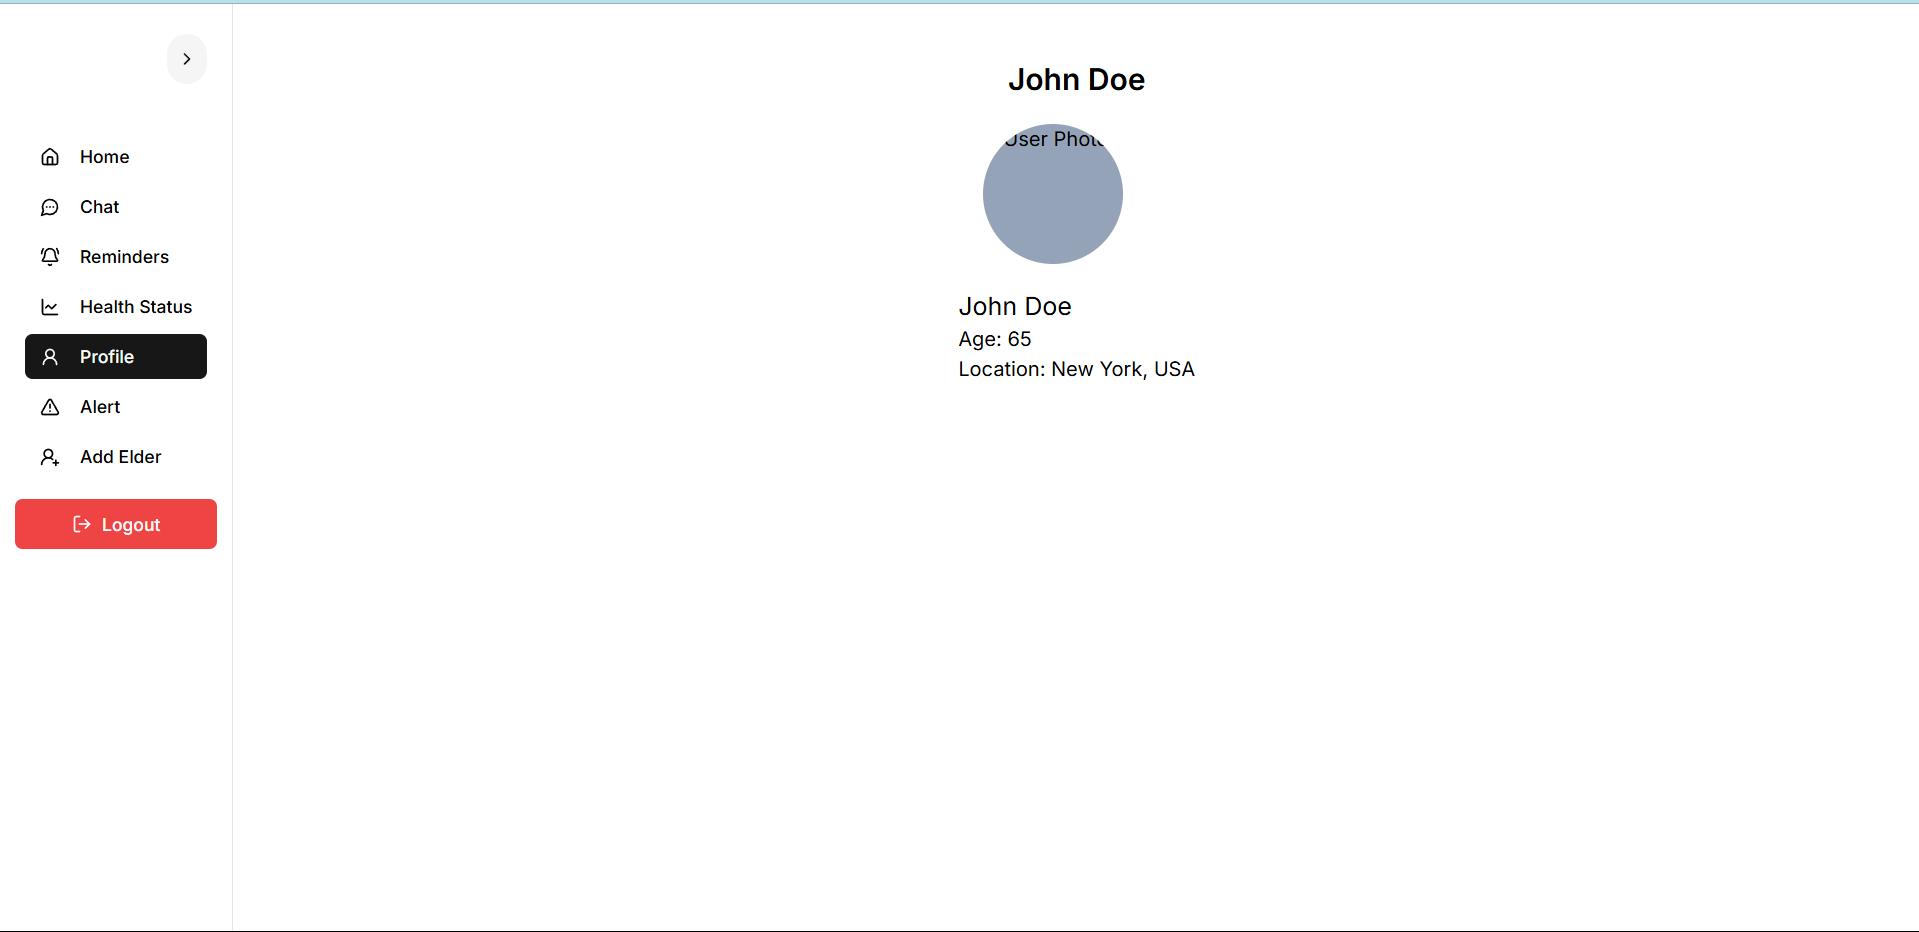
\includegraphics[width=0.9\textwidth]{profile.png}
        \caption{Profile}
        \label{fig:profile}
    \end{minipage}
    \vspace{5pt}
\end{figure}

\begin{figure}
    \centering
    \begin{minipage}{\textwidth}
        \centering
        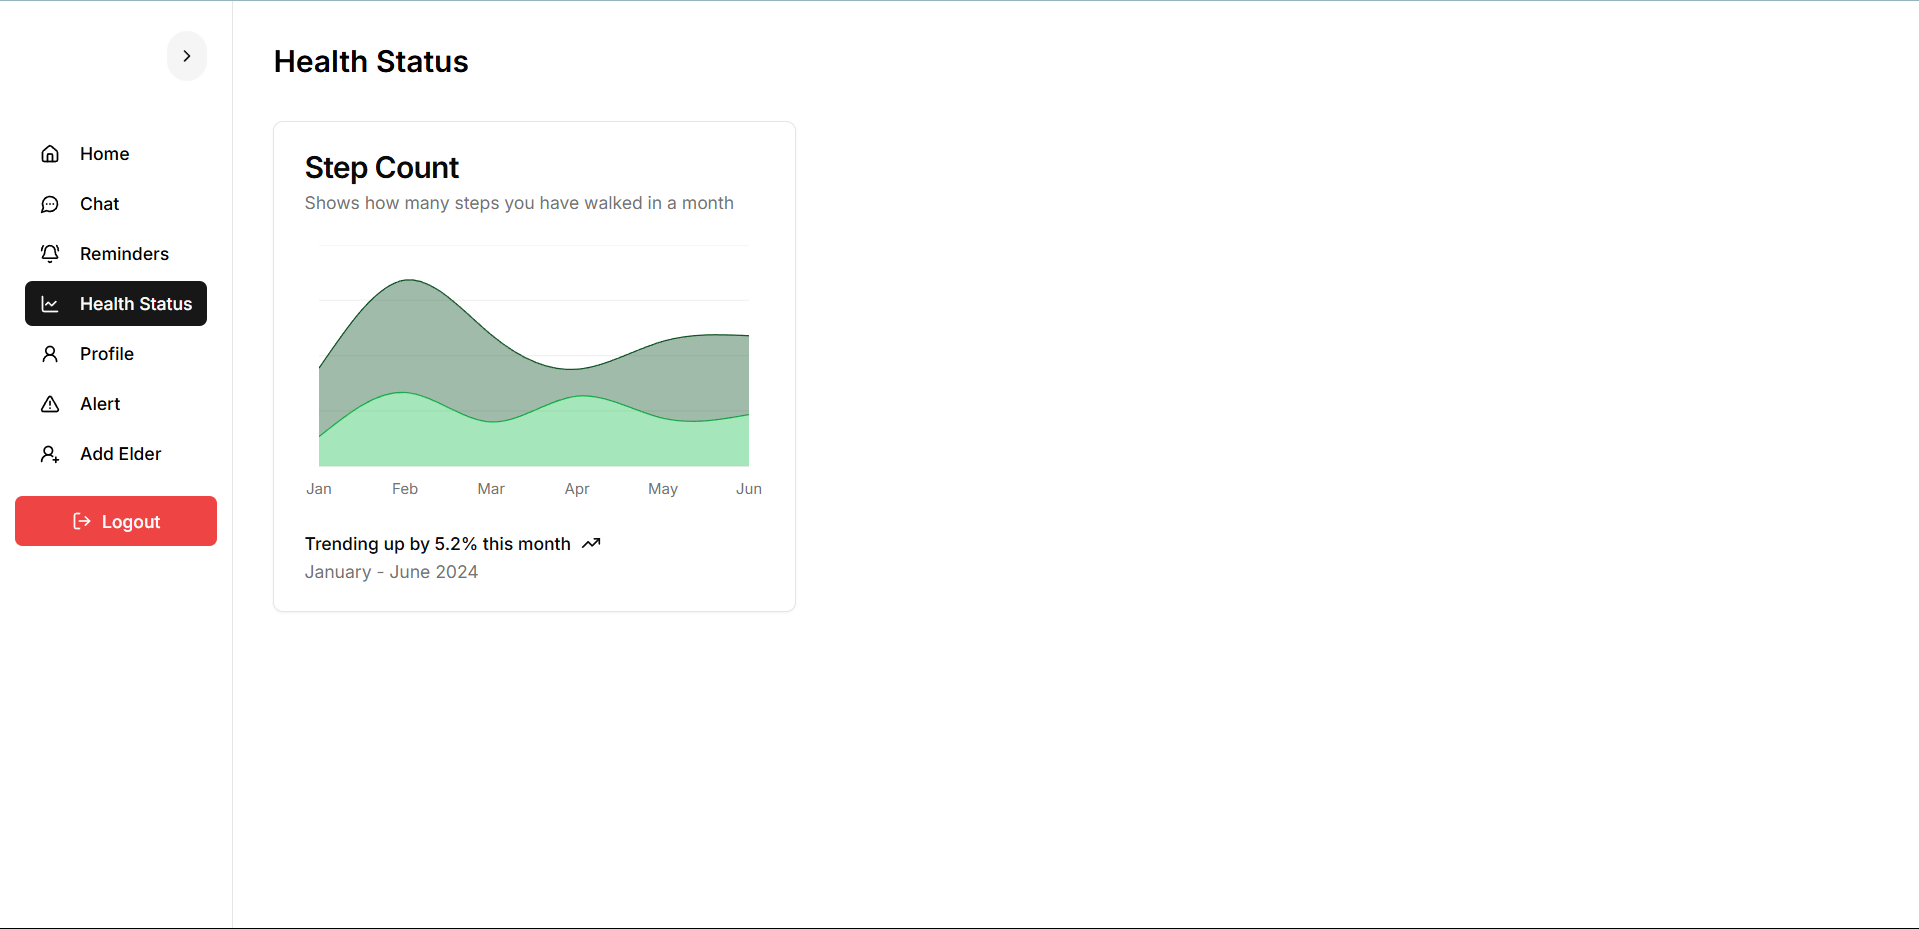
\includegraphics[width=0.9\textwidth]{health data.png}
        \caption{Health Status}
        \label{fig:health_status}
    \end{minipage}
    \vspace{5pt}
    \begin{minipage}{\textwidth}
        \centering
        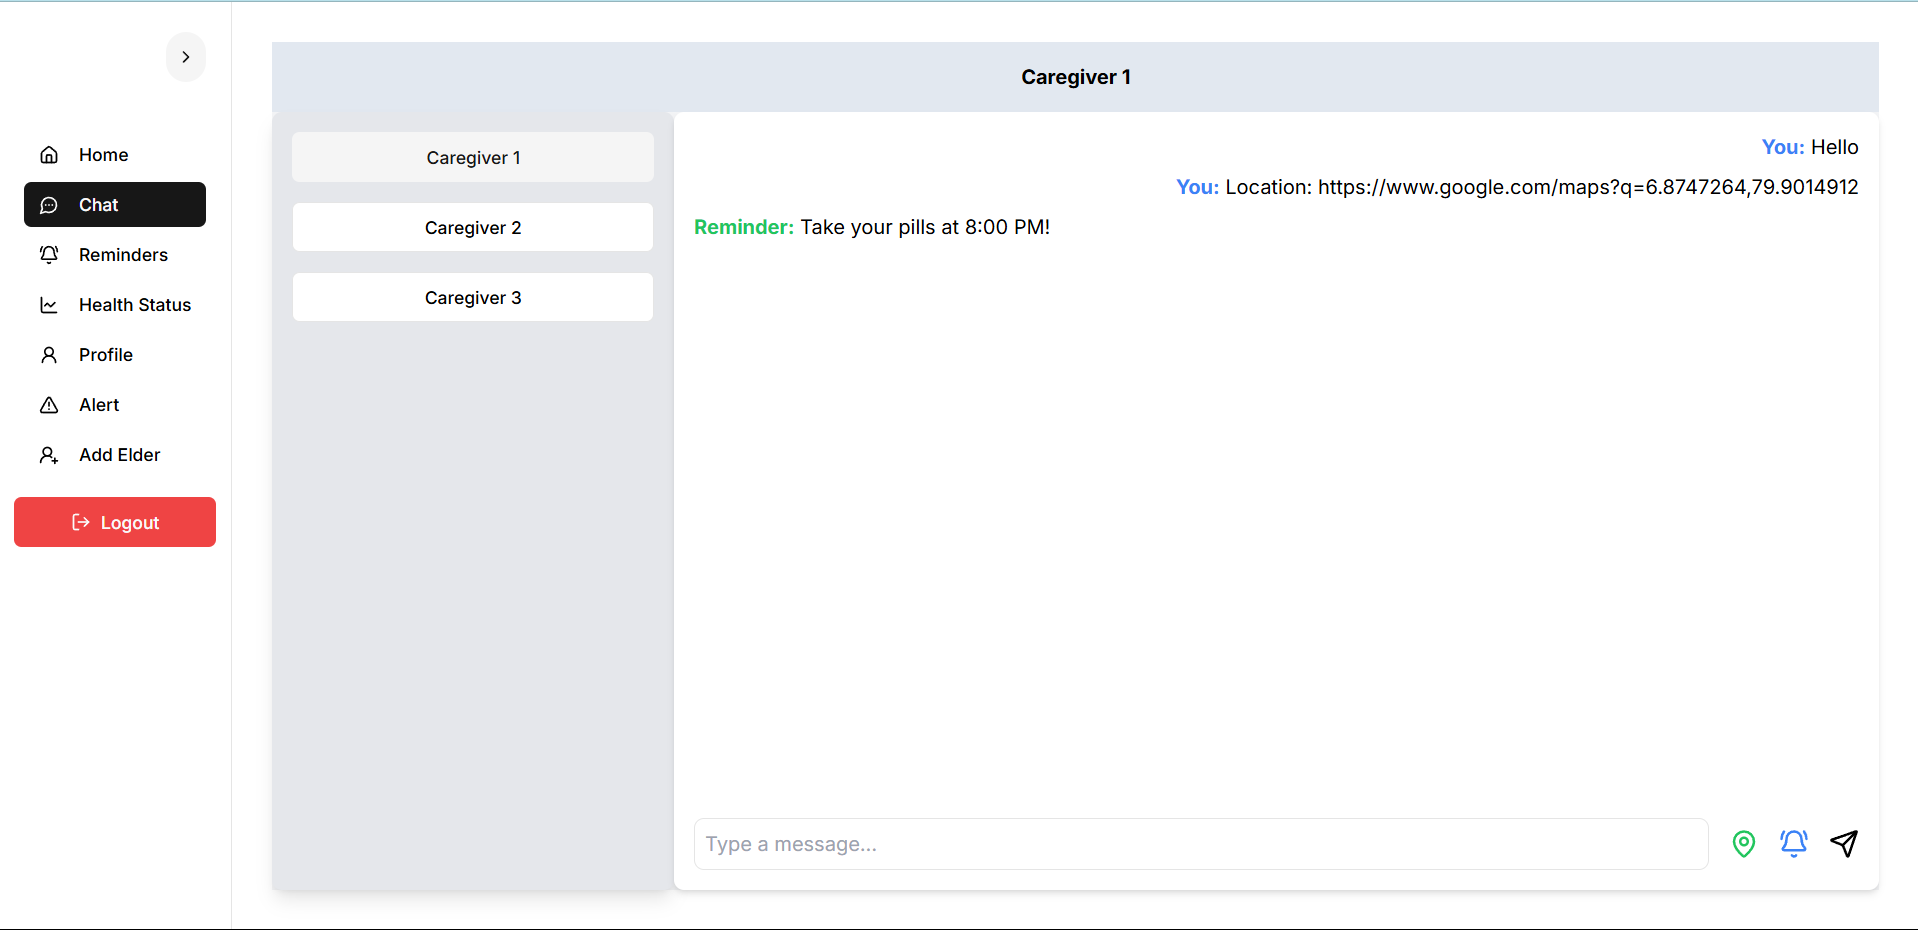
\includegraphics[width=0.9\textwidth]{chat.png}
        \caption{Chat}
        \label{fig:chat}
    \end{minipage}
    \vspace{5pt}
    \begin{minipage}{\textwidth}
        \centering
        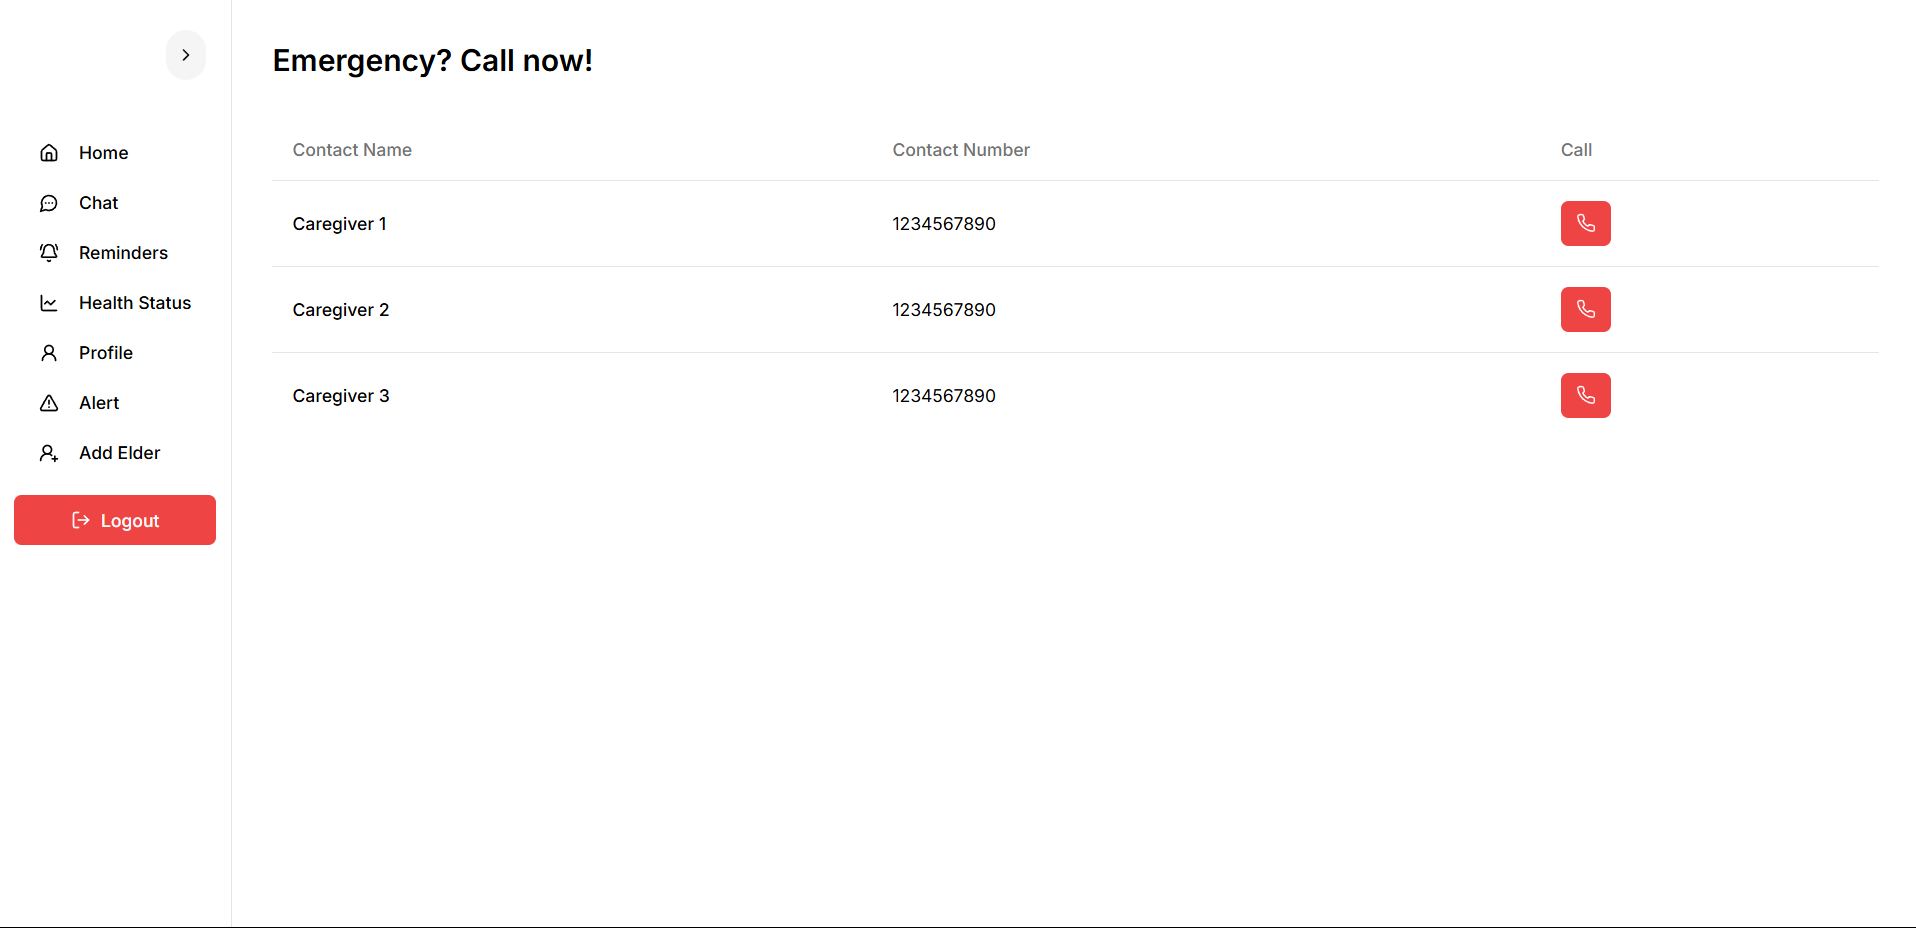
\includegraphics[width=0.9\textwidth]{emergency contact.png}
        \caption{Emergency Call}
        \label{fig:emergency_call}
    \end{minipage}
    \vspace{5pt}
\end{figure}
\newpage
% \begin{figure}
%   \centering
%   % Requires \usepackage{graphicx}
%   \includegraphics[width=6.4in]{dashboard}\\
%   \caption{Dashboard: This is the title of the figure}\label{fig:dashboard}
% \end{figure}



\newpage
%%%%%%%%%%%%%%%%%%%%%%%%%%%%%%%%%%%%%%%%%%%%%%%%%%%%%%%%%%%%%%%%%%%%%%

%%%%%%%%%%%%%%%%%%%                 conclusion.tex}
\chapter{Limitations, Recommendations, and Conclusion}
\section{Introduction}
This section provides a comprehensive overview of the Limitations, Recommendations, and Conclusion of the Elder Care Connect project. As with any system, there are inherent limitations that impact its functionality, ranging from technical constraints to user adoption challenges. Addressing these constraints, we offer recommendations for future enhancements to improve system efficiency, security, and user experience. Finally, we summarize the project’s significance and potential impact on elderly care services, highlighting the value it brings to caregivers and elderly individuals alike.
\section{Limitations}
While the proposed Progressive Web Application (PWA) offers significant advantages for elderly individuals living alone, there are certain limitations that need to be addressed:
\begin{itemize}
    \item \textbf{Internet Dependency:} The real-time health monitoring and emergency alert system require a stable internet connection, which may not always be available in remote areas.
    \item \textbf{Device Compatibility:} The effectiveness of health tracking depends on integration with wearable devices, which may not be universally available or compatible with all elderly users.
    \item \textbf{User Adoption and Digital Literacy:} Elderly individuals with limited technological experience may find it difficult to navigate the application without external assistance.
    \item \textbf{Privacy and Security Concerns:} Handling sensitive health data requires robust encryption and authentication mechanisms to ensure data security and compliance with healthcare regulations.
    \item \textbf{Healthcare Integration Challenges:} The effectiveness of the app depends on cooperation from healthcare providers, which may vary based on location and medical policies.
\end{itemize}
\section{Recommendations}
To address these limitations and enhance the application's usability, the following recommendations are proposed:
\begin{itemize}
    \item \textbf{Offline Functionality:} Implement local storage and caching to enable essential features such as medication reminders and emergency contact access even in offline mode.
    \item \textbf{Improved Device Support:} Expand compatibility with a wide range of wearable health devices to accommodate diverse user needs.
    \item \textbf{User Training and Support:} Develop easy-to-follow tutorials and provide customer support services to help elderly users and caregivers navigate the application.
    \item \textbf{Enhanced Security Measures:} Strengthen encryption techniques, implement multi-factor authentication, and ensure compliance with healthcare data regulations.
    \item \textbf{Healthcare Partnerships:} Collaborate with medical institutions to facilitate seamless integration with healthcare services and ensure accurate monitoring of user health data.
    \item \textbf{Customization Options:} Allow caregivers and family members to personalize alerts, notifications, and interface settings to better suit individual user needs.
\end{itemize}
\section{Conclusion}
The development of the ElderCare Connect application aims to enhance the safety, health monitoring, and social well-being of elderly individuals living alone. By leveraging real-time health tracking, emergency alerts, and social engagement features, the application ensures improved care and independent living for elderly users. The integration of wearable devices and Progressive Web Application (PWA) technology provides accessibility across multiple devices while maintaining offline support.\\
Despite certain limitations such as internet dependency and healthcare integration challenges, the recommended solutions—offline capabilities, improved device support, and enhanced security measures—can significantly enhance the application's effectiveness. With further development and collaboration with healthcare providers, this application has the potential to revolutionize elderly care, offering peace of mind to families and caregivers while promoting independent living for elderly individuals.




\newpage
\newpage









\newpage
%%%%%%%%%%%%%%%%%%%%%%%%%%%%%%%%%%%%%%%%%%%%%%%%%%%%%%%%%%%%%%%%%%%%%%

\bibliographystyle{IEEEtran}
\bibliography{references} 

\end{document}
